\chapter{Testowalność oprogramowania}
\section{Pojęcie testowalności i pielęgnowalności oprogramowania}
Jako analityk testowy z pojęciem testowalności oprogramowania autor spotyka się już od początku pracy w branży. Termin „testowalność oprogramowania” \footnote{Definicja testowalności według standardu ISO9126}  według definicji ISTQB \footnote{International Software Qualification Board}  i ISO9126, to najkrócej mówiąc właściwość tego oprogramowania umożliwiająca testowanie go po zmianach. Termin ten ściśle powiązany jest także z innym pojęciem ze słownika testerskiego – pielęgnowalnością. A pielęgnowalność \footnote{Definicja pielęgnowalności według ISTQB} , to łatwość, z którą oprogramowanie może być modyfikowane w celu naprawy defektów, dostosowania do nowych wymagań, modyfikowane w celu ułatwienia przyszłego utrzymania lub dostosowania do zmian zachodzących w jego środowisku.

\section{Czy testowanie jest potrzebne?}
Po co tak w ogóle właściwie testować oprogramowanie? Czy testowanie jest potrzebne? Jak dużo testów należy przeprowadzić, aby testowanie było wystarczająco skuteczne? To są pytania, które mogą być tematem osobnej pracy, w tym rozdziale poruszymy tylko pojęcia, które zaostaną wykorzystane w dalszej części tej pracy.

Człowiek, jako istota żywa i omylna, może popełnić podczas pracy \textbf{błąd}, czyli inaczej – \textbf{pomyłkę}. Pomyłka w pracy programisty może skutkować pojawieniem się \textbf{defektu} (usterki, pluskwy) w kodzie programu, bądź w dokumencie. Do tej pory nic się nie dzieje złego, ale jeżeli kod programu, który posiada w sobie taki defekt, zostanie wykonany, system może nie zrobić tego, co od niego wymagamy, lub wykonać to niezgodnie z założeniami, czyli inaczej rzecz ujmując, ulegnie \textbf{awarii}. 

Defekty powstają, ponieważ jak już wspomnieliśmy wcześniej, ludzie są omylni. Ale pomyłka człowieka, to nie jedyny powód awarii systemów. Mogą one być również spowodowane przez warunki środowiskowe, takie jak promieniowanie, pole magnetyczne i elektryczne, czy nawet zanieczyszczenia środowiska.

Czy testowanie pomaga nam w całkowitym uniknięciu awarii systemów? Na pewno nie, ale pozwala je drastycznie ograniczyć. Za pomocą zestawu testów możemy zmierzyć jakość oprogramowania wyrażoną przez ilość znalezionych usterek oraz możemy budować zaufanie do jakości oprogramowania, jeżeli jako osoby testujące znajdujemy ich mało, bądź nie znajdujemy ich wcale.

I tutaj najważniejsza teza: \textbf{Testowanie samo w sobie nie poprawia jakości oprogramowania!} Dopiero umiejscowienie defektu w kodzie programu (zdebugowanie) oraz naprawa tego błędu przez programistę poprawi nam tą jakość. Poniżej na rysunku widzimy tabelę (słynną już, gdyż korzysta z niej wielu trenerów prowadzących kursy z testowania oprogramowania), jak testowanie na poszczególnych etapach wytwarzania oprogramowania wpływa na koszty projektu.

\begin{table}[]
\centering
\caption{Koszty znalezienia błędu na poszczególnych etapach projektu}
\label{tab:koszty_bledu}
\begin{tabular}{|l|l|}
\hline
\textbf{Błąd znaleziony podczas} & \textbf{Szacowany koszt} \\ \hline
Projektowania & 1 PLN	\\ \hline
Inspekcji (przeglądu) & 10 PLN	\\ \hline
W początkowej fazie produkcji & 100 PLN	\\ \hline
Podczas testów systemowych & 1000 PLN	\\ \hline
Po dostarczeniu produktu na rynek & 10000 PLN	\\ \hline
Kiedy produkt musi zostać wycofany z rynku & 100000 PLN	\\ \hline
Kiedy produkt musi zostać wycofany z rynku po wyroku sądowym & 1000000 PLN	\\ \hline
\end{tabular}
\end{table}

Z zestawienia jasno wynika, że praca testerów nie zaczyna się gdy program już jest napisany przez programistów, a zaczyna się już w najwcześniejszej fazie projektu, na etapie projektowania.

\section{Obszary testowe}
Idealnie byłoby mieć możliwość przetestować każdą linijkę kodu. Autor zdaje sobie sprawę, że w wielu przypadkach jest to niemożliwe, a nawet bezcelowe, więc dopuszcza się możliwość ograniczenia testowania do kluczowych elementów kodu źródłowego, czy kluczowych funkcjonalności. Zwykle nie jest potrzebne testowanie \textit{setterów}, \textit{getterów}, czy funkcji należących do standardowych bibliotek (zapewne zostały przetestowane już podczas ich tworzenia). 

Bazując na publikacji \textit{"Learning Android Application Testing"\cite{bib:android:testing:learning}} autor wyróżnił następujące trzy główne obszary testowania:

\begin{itemize}
\item{Cykle życia aktywności}

Należy przetestować, czy aktywność przechodzi prawidłowo przez swoje cykle życia. Jeżeli od tworzonej aplikacji wymagamy, żeby zachowywała swój stan podczas \texttt{onPause()} albo \texttt{onDestroy()} i poźniej odtwarzała zachowany stan podczas wykonywania funkcji \texttt{onCreate()}, wtedy powinniśmy napisać testy pokrywające wszystkie te przypadki i sprawdzające, czy zachowany status został odtworzony poprawnie. Trzy główne pętle do przetestowania znajdują się na poniższym schemacie:
\begin{figure}[!htb]
    \centering
    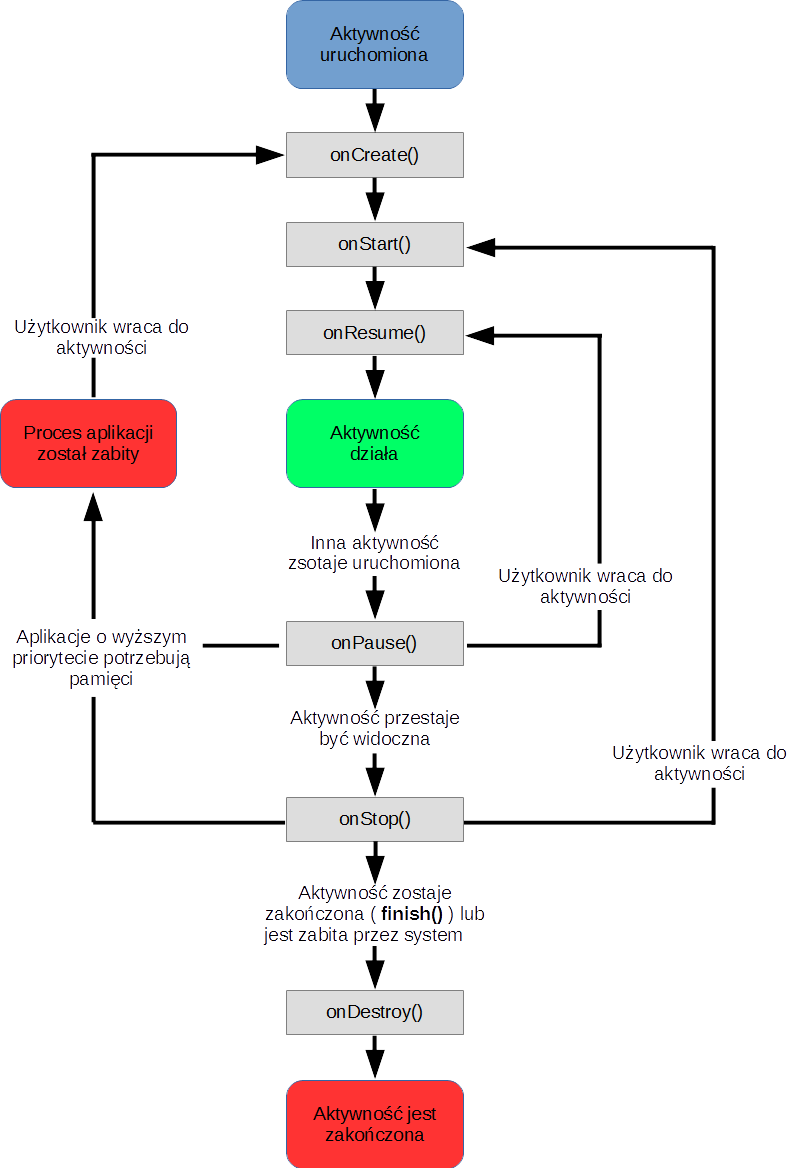
\includegraphics[width=10cm]{imgs/ch2_activity_lifecycle.png}
    \caption{Cykl życia \textit{Activity}. Źródło: \href{http://developer.android.com/reference/android/app/Activity.html}{Dokumentacja Android}}
    \label{fig:sample_figure}
\end{figure} 


\item{Dostęp do baz danych i do systemu plików}

Należy sprawdzić, czy operacje dostępowe przeprowadzane są poprawnie, a jeżeli nie, to czy również poprawnie działa obsługa błędów. Testować to można na kilka sposobów: albo na niskim poziomie, izolując warstwę użytkownika, albo bezpośrednio z aplikacji. Do testowania na niskim poziomie możemy wykorzystywać dostarczane przez framework Androida w pakiecie \texttt{android.test.mock} \textit{zaślepki}\footnote{Zaślepka (stub) - szkieletowa albo specjalna implementacja modułu używana podczas produkcji lub testów innego modułu, który tę zaślepkę wywołuje albo jest w inny sposób od niej zależny. Zaślepka zastępuje wywoływany moduł. [wg. IEEE 610]}

Według dokumentacji Android\cite{website:android:manual} możliwe są następujące opcje przechowywania danych:

- \textit{Shared Preferences}, czyli zachowywanie podstawowych danych w parach klucz - wartość,

- pamięć wewnętrzna urządzenia - do zachowywania danych niepublicznych,

- zewnętrzna karta pamięci - do zachowywania danych publicznych,

- baza danych SQLite - do przechowywania danych w prywatnej bazie danych,

- zasoby sieciowe - jako baza danych współdzielona pomiędzy urządzeniami.

Wszystkie te opcje korzystają ze wspólnego zestawu funkcji\footnote{Na przykład do obsługi plików używamy \textit{getFileDir(), getDir(), deleteFile()} itp.}, które tester powinien wziąć pod uwagę przy tworzeniu przypadków testowych.

\item{Fizyczną charakterystykę urządzenia}

Android został zaprojektowany do pracy na wielu różnych typach urządzeń, od telefonów do tabletów i telewizorów. Deweloperzy muszą tolerować pewną zmienność zachowań projektowanych funkcji i zapewnić elastyczny interfejs użytkownika, który dostosowuje się do różnych konfiguracji ekranu czy sieci.

Należy sprawdzić, czy aplikacja działa poprawnie na wszystkich urządzeniach, na których można ją uruchomić. To, że działa świetnie na smartfonie, nie zanczy że działa poprawnie na tablecie, a to że działa na smartfonie jednej firmy nie wyklucza awarii na tym samym urządzeniu wyprodukowanym przez kogoś innego. Elementy, które powinniśmy testować w tym zakresie, to:

- możliwości sieciowe,

- rozdzielczość ekranu,

- gęstość ekranu,

- rozmiar ekranu,

- czułość sensorów,

- klawiaturę i inne urządzenia wejściowe,

- lokalizację GPS,

- zewnętrzne karty pamięci.

Android framework dostarcza rozwiązań pozwalających pewne rzeczy dostosowywać automatycznie, ale nie zwalnia to projektantów przed wykonaniem zestawu niezbędnych testów również w tym obszarze.

\end{itemize}

\section{Rodzaje testów}
Proces testowania może zostać wprowadzony na każdym etapie tworzenia aplikacji, w zależności od wybranej strategii testu. Jednakże, jak już autor wspomniał wcześniej, najlepiej jest rozpoczynać testowanie tak szybko jak to jest możliwe, w możliwie najwcześniejszym stadium projektu. Nawet jeżeli nie wszystkie wymagania systemowe zostały uzgodnione, a proces pisania oprogramowania się jeszcze nie rozpoczął. Już sam etap tworzenia dokumentacji i \textit{requirementów} może zostać poddany testowaniu. Pozwala to unikać błędów już na etapie wczesnego projektowania, a które mogłyby implikować proces tworzenia przez długi czas.

Rozpoznaje się kilka poziomów testowania, w zależności od modelu zarządzania projektem. Jeżeli weźmiemy pod uwagę model V przedstawiony na schemacie \ref{fig:model_v}, wyróżnić możemy cztery główne interesujące nas obszary:

\begin{itemize}
\item
testy jednostkowe (\textit{Unit tests})
\item
testy integracyjne
\item
testy systemowe
\item
testy akceptacyjne

\end{itemize}

\begin{figure}[!htb]
    \centering
    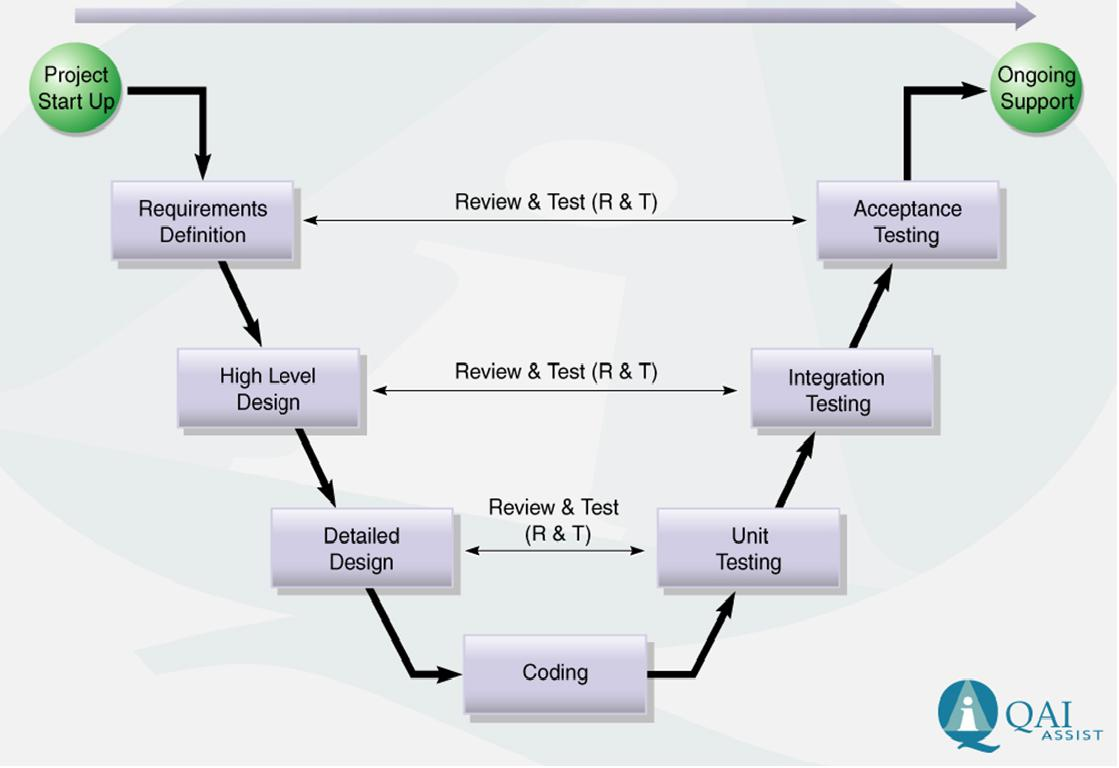
\includegraphics[width=10cm]{imgs/ch2_model_v.jpg}
    \caption{Model V - najpopularniejszy model zarządzania projektem informatycznym (\textit{V\-model}). Źródło: \href{http://www.projectinsight.net/blogs/it-project-management-solutions/the-quot-v-quot-model-by-cameron-watson}{"V" Model opisany przez Cameron Watson}}
    \label{fig:model_v}
\end{figure} 

\paragraph{Testy jednostkowe (modułowe)}


"Testy modułowe polegają na wyszukiwaniu błędów i weryfikacji funkcjonalności oprogramowania (np. modułów, programów, obiektów, klas), które można testować
oddzielnie. Może być wykonywane w izolacji od reszty systemu, w zależności od kontekstu cyklu rozwoju oprogramowania i od samego systemu. Można podczas nich użyć zaślepek, sterowników testowych oraz symulatorów." \cite{bib:sylabus:foundation}

Mogą one zawierać testy funkcjonalności oraz niektórych atrybutów niefunkcjonalnych, takich jak stopień wykorzystania zasobów (np. wycieków pamięci) lub odporności. Wlicza się w nie również testy strukturalne - pokrycia linii kodu, decyzji lub gałęzi. Do projektowania przypadków testowych bardzo przydatna jest specyfikacja fumkcji. Wtedy jest możliwość zaprojektowania testów zanim zostanie napisany kod programu (tzw. "wytwarzanie sterowane testowaniem", opisane szerzej w sekcji \ref{test_driven_development}. "Testy modułowe zwykle wykonuje się mając dostęp do kodu źródłowego i przy wsparciu środowiska rozwojowego (np. bibliotek do testów jednostkowych, narzędzi do debagowania) oraz, w praktyce, zwykle angażują też programistę, który jest autorem kodu. Usterki są usuwane jak tylko zostaną wykryte, bez formalnego zarządzania nimi."   \cite{bib:sylabus:foundation}

Najczęściej wykorzystywanem frameworkiem testowym dla Unit Testów pod Androidem jest środowisko JUnit. To proste i użyteczne środowisko, pozwalające automatyzować testy jednostkowe, zostało zaprojektowane przez Ericha Gamma\footnote{Erich Gamma - szwajcarski informatyk, współautor książki "Wzorce projektowe: elementy oprogramowania obiektowego wielokrotnego użytku". Wspólnie z Kentem Beckiem napisał narzędzie do tworzenia testów jednostkowych JUnit. Rozwijał także środowisko Eclipse.} i Kenta Becka i wydane na licencji \textit{open source}.

Głównie badaniem tego rodzaju testów autor zajmował się będzie w części doświadczalnej pracy magisterskiej.

\paragraph{Testy integracyjne}

"Testy integracyjne sprawdzają interfejsy pomiędzy modułami, interakcje z innymi częściami systemu (takimi jak system operacyjny, system plików i sprzęt) oraz interfejsy pomiędzy systemami. "\cite{bib:sylabus:foundation}

Wykonuje je się zwykle, jeżeli jest tylko jest możliwość przetestowania integracji gotowych już modułów (napisanych i przetestowanych testami jednostkowymi). Pojęcie testowania integracynego można rozszerzyć również na testowanie integracji pomiędzy różnymi systemami, a nawet produktami różnych producentów. 

\paragraph{Testy systemowe}

"Testy systemowe zajmują się zachowaniem systemu/produktu. Zakres testów powinien być jasno określony w głównym planie testów oraz w planach testów poszczególnych poziomów. [...] Testy systemowe mogą zawierać testy oparte na ryzyku lub wymaganiach, procesie biznesowym, przypadkach użycia lub jeszcze innych wysokopoziomowych opisach słownych lub modelach zachowania systemu, interakcji z systemem operacyjnym i zasobami systemowymi."\cite{bib:sylabus:foundation}

Dąży się do tego, aby środowisko testowe w przypadku testów systemowych było maksymalnie zbliżone do środowiska docelowego, w którym projektowana aplikacja ma działać. Optymalnie byłoby pokryć wszystkie możliwe konfiguracje sprzętowe, aczkolwiek z wielu powodów, głównie finansowych, firmy skupiają sie na najczęściej wykorzystywanych przez użytkownikach urządzeniach. 

\paragraph{Testy akceptacyjne}

"Celem testów akceptacyjnych jest nabranie zaufania do systemu, jego części lub pewnych atrybutów niefunkcjonalnych. Wyszukiwanie usterek nie jest tym, na czym skupiają się testy akceptacyjne. Mogą one oceniać gotowość systemu do wdrożenia i użycia, chociaż nie muszą być ostatnim poziomem testowania. Na przykład może po nich następować testowanie integracji systemów w większej skali."\cite{bib:sylabus:foundation}

Odpowiedzialność za testy akceptacyjne, w przeciwieństwie do testów opisanych w poprzednich paragrafach, leży po stronie klientów. Zwykle testy akceptacyne dzieli się na dwa etapy: testy \textit{alfa} oraz \textit{beta}. Testy \textit{alfa} przeprowadzane są przez przyszłych użytkowników w siedzibie producenta, natomiast \textit{beta} - w środowisku docelowym. W praktyce producenci oprogramowania przekazują darmowe wersje swoich aplikacji o ograniczonych możliwościach, oczekując w zamian od użytkowników raportowania błędów lub propozycji usprawnień, bądź uzyskując to raportowanie automatycznie, kiedy aplikacja sama wysyła do producenta informację o zaistniałych defektach.

\section{Wytwarzanie sterowane testowaniem - \textit{Test Driven Development}}
\label{test_driven_development}
Technika wytwarzania sterowanego zarządzaniem zyskuje coraz więcej popularności. Związane to jest pośrednio z nowymi modelami zarządzania projektami informatycznymi opartymi na metodykach zwinnych, w tym Agile\footnote{Agile software development) – grupa metodyk wytwarzania oprogramowania opartego na programowaniu iteracyjno-przyrostowym, powstałe jako alternatywa do tradycyjnych metod typu waterfall. Najważniejszym założeniem metodyk zwinnych jest obserwacja, że wymagania odbiorcy (klienta) często ewoluują podczas trwania projektu. Oprogramowanie wytwarzane jest przy współpracy samozarządzalnych zespołów, których celem jest przeprowadzanie procesów wytwarzania oprogramowania. (Źródło: Wikipedia) }. W założeniu podejście takie pozwala:

\begin{itemize}
\item znaleźć więcej błędów na wcześniejszym etapie procesu developmentu;
\item świadomie zrobić zmiany wtedy, kiedy są potrzebne;
\item łatwo wykonać testy regresywne bazując na wcześniej napisanych procedurach;
\item przedłużyć żywotność kodu.
\end{itemize}

Jeżeli istnieją unit testy i pokrywają znaczącą część kodu źródłowego, wtedy jasne jest, że więcej błędów zostanie znalezionych i poprawionych. W ten sam sposób przy podejściu \textit{Test Driven Development (TDD)} można wywnioskować, że skoro unit testy są już napisane, z dużym prawdopodobieństwem pokrycie kodu będzie zadowalające. Co więcej, raz napisane testy można wykorzystywać do przeprowadzania testów regresywnych, aby się upewnić, czy zmiany w naszym oprogramowaniu zgodne są z założeniami i wymaganiami systemu.

Unit testy w podejściu TDD zapewniają, że jakość oprogramowania nie jest oparta na domysłach i przekonaniu programistów, a na rzetelnych raportach. Bez obaw można dokonywać modyfikacji takich, jak zmiana serwera baz danych, zmiana designu, interfejsu użytkownika, czy nawet API. Jeżeli wszystkie testy zostaną sprawdzone pozytywnie - oprogramowanie będzie działać nadal bezbłędnie.

Podsumowując, podejście TDD znacznie zwiększa nam więc testowalność i pielęgnowalność aplikacji. 

\section{Wytwarzanie sterowane zachowaniem - \textit{Behaviour Driven Development}}
\label{behaviour_driven_development}


\section{Alternative testing tactics}

\section{Testowalność aplikacji androidowych}
Jak to jest więc z tą testowalnością oprogramowania dla Android? Czy aktualna struktura stosowana w większości aplikacji jest testowalna? Czy, o ile nie jest, da się tak poprawić strukturę programów, aby były bardziej testowalne niż obecnie? Jak nie psuć wcześniej działających części aplikacji wprowadzanymi zmianami w kodzie? Jak w ogóle wykrywać takie sytuacje, gdy coś przypadkowo zepsuliśmy? Jak dzielić odpowiedzialność pomiędzy częściami naszego oprogramowania? Jak rozwiązać problem zbyt dużego sprzężenia zarówno w naszym kodzie, jak i pomiędzy naszym kodem i frameworkiem androidowym \footnote{Sprzężenie (\textit{ang. coupling}) jest miarą jak bardzo obiekty, podsystemy lub systemy zależą od siebie nawzajem.}? No i w ogóle, jak testować aplikacje dla Androida poprawnie?

Na te pytania autor postara się odpowiedzieć w dalszej części pracy.
%tutaj przykłady jak użyć poszczególnych konstrukcji
%Przykładowy rysunek \ref{fig:sample_figure}. Prztykładowa tabela %\ref{tab:sample_table}. Przykładowy odnośnik do bibliografi \cite{bib:kowalski_2015}. \textbf{Powodzenia!}


%\begin{figure}[!htb]
%    \centering
%    \includegraphics[width=10cm]{imgs/sample_figure.jpg}
%    \caption{Przykłady rysunek}
%    \label{fig:sample_figure}
%\end{figure} 

%\begin{table}[]
%\centering
%\caption{Przykładowa tabela}
%\label{tab:sample_table}
%\begin{tabular}{|l|l|}
%\hline
%\textbf{Nazwa} & \textbf{Wartość} \\ \hline
%Test           & 1.2              \\ \hline
%Kwiatek        & 5                \\ \hline
%\end{tabular}
%\end{table}